\documentclass[letterpaper, 11pt]{article}
    \usepackage[margin=0.9in]{geometry}
    \usepackage{graphicx, hyperref, enumitem, booktabs}
    \usepackage{cancel, verbatim}
    % rubber: set program xelatex
    \usepackage[calc,physics,stix]{bccho}

    \usepackage{tocloft}
    \usepackage{etoc}
    \usepackage[margin=1cm]{caption}
    \usepackage{subcaption}
    \usepackage{float}
    % rubber: setlist arguments --shell-escape
    \usepackage{minted}
    \usepackage[linewidth=0pt]{mdframed}

    \definecolor{bg}{rgb}{0.95, 0.95, 0.95}
    \BeforeBeginEnvironment{minted}{\begin{mdframed}[backgroundcolor=bg]}
    \AfterEndEnvironment{minted}{\end{mdframed}}

    % \renewcommand{\thefigure}{\thesection.\arabic{figure}}
    \captionsetup[figure]{labelfont={it,bf}}
    \captionsetup[table]{labelfont={it,bf}}
    \captionsetup[subfigure]{labelfont={it}}

% Begin document

\begin{document}
    \begin{center}
        \large
        \textsc{\textbf{ELE 302 -- Independent Project Write-Up}} \vspace{5pt}

        \normalsize
        TJ Smith \hspace{1cm} Byung-Cheol Cho \\
        (Bench 207) \vspace{5pt}

        \emph{Due May 19, 2017}
        \normalsize
    \end{center}

\section{Overview}
The aim of this project was to build a robot capable of playing basic ping pong. Prior to beginning this project, we established four ideal objectives for the end product:
\begin{enumerate}[label=\textbf{\arabic*.}]
    \item Track a ping pong ball, estimate its trajectory and predict the location where the ball will land
    \item Determine (1) when it is the robot's turn to hit the ball and (2) when the ball will hit the net or leave the playing area
    \item Move the robot to the required location before the ball bounces twice and hit the ball back over the net
    \item Avoid leaving the playing field (area enclosed by table and net)
\end{itemize}
By Demo Day, we had implemented the hardware and software to achieve objectives 1, 3 and the first half of objective 2, and we had the capability of achieving the remainder of the objectives had we decided to implement them in software.

We used two Pixy cameras (CMUcam5) placed a fixed distance apart on the robot to triangulate the location of a bright red ball in three-dimensional coordinates. Once the camera system had collected enough data points to accurately predict all future positions of the ball until the second bounce, the robot moved to a location where the ball would bounce to the center of a paddle attached to its side, and provided a brief flick to the paddle to return the ball.

The speed and flexibility of movement we needed (we had to move up to 3 feet in less than half a second) required us to abandon the chassis used for our previous speed control and navigation assignments and adopt the large and powerful omni-wheel drive used by Ethan Gordon and Luke Pfleger in 2016. We used an accelerometer and gyroscope for dead reckoning of position (we could no longer use wheel rotation tracking because of slippage). In addition, we continued to use the PSoC 5LP because of its extensive motor control capacity (we required four PWM modules) while adding a Raspbery Pi 3 because of the intensive computation we expected to require for ball tracking and trajectory estimation.

\section{Theory}

\subsection{Trajectory estimation}
%TODO: BC: write all the equations

\subsection{Omni-drive}
%TODO: TJ: give BC equations and BC typesets them

\section{Hardware}
%TODO: BC: photos front, side, top of robot
%TODO: BC: block diagram

Figure~\ref{fig:blockdiagram} shows a block diagram of the hardware set-up pertinent to autonomous navigation (see previous write-up for the hardware for speed control, such as the motor board, main driving motor, Hall effect sensor and Hall effect sensor board).
\begin{figure}[ht]
    \centering
    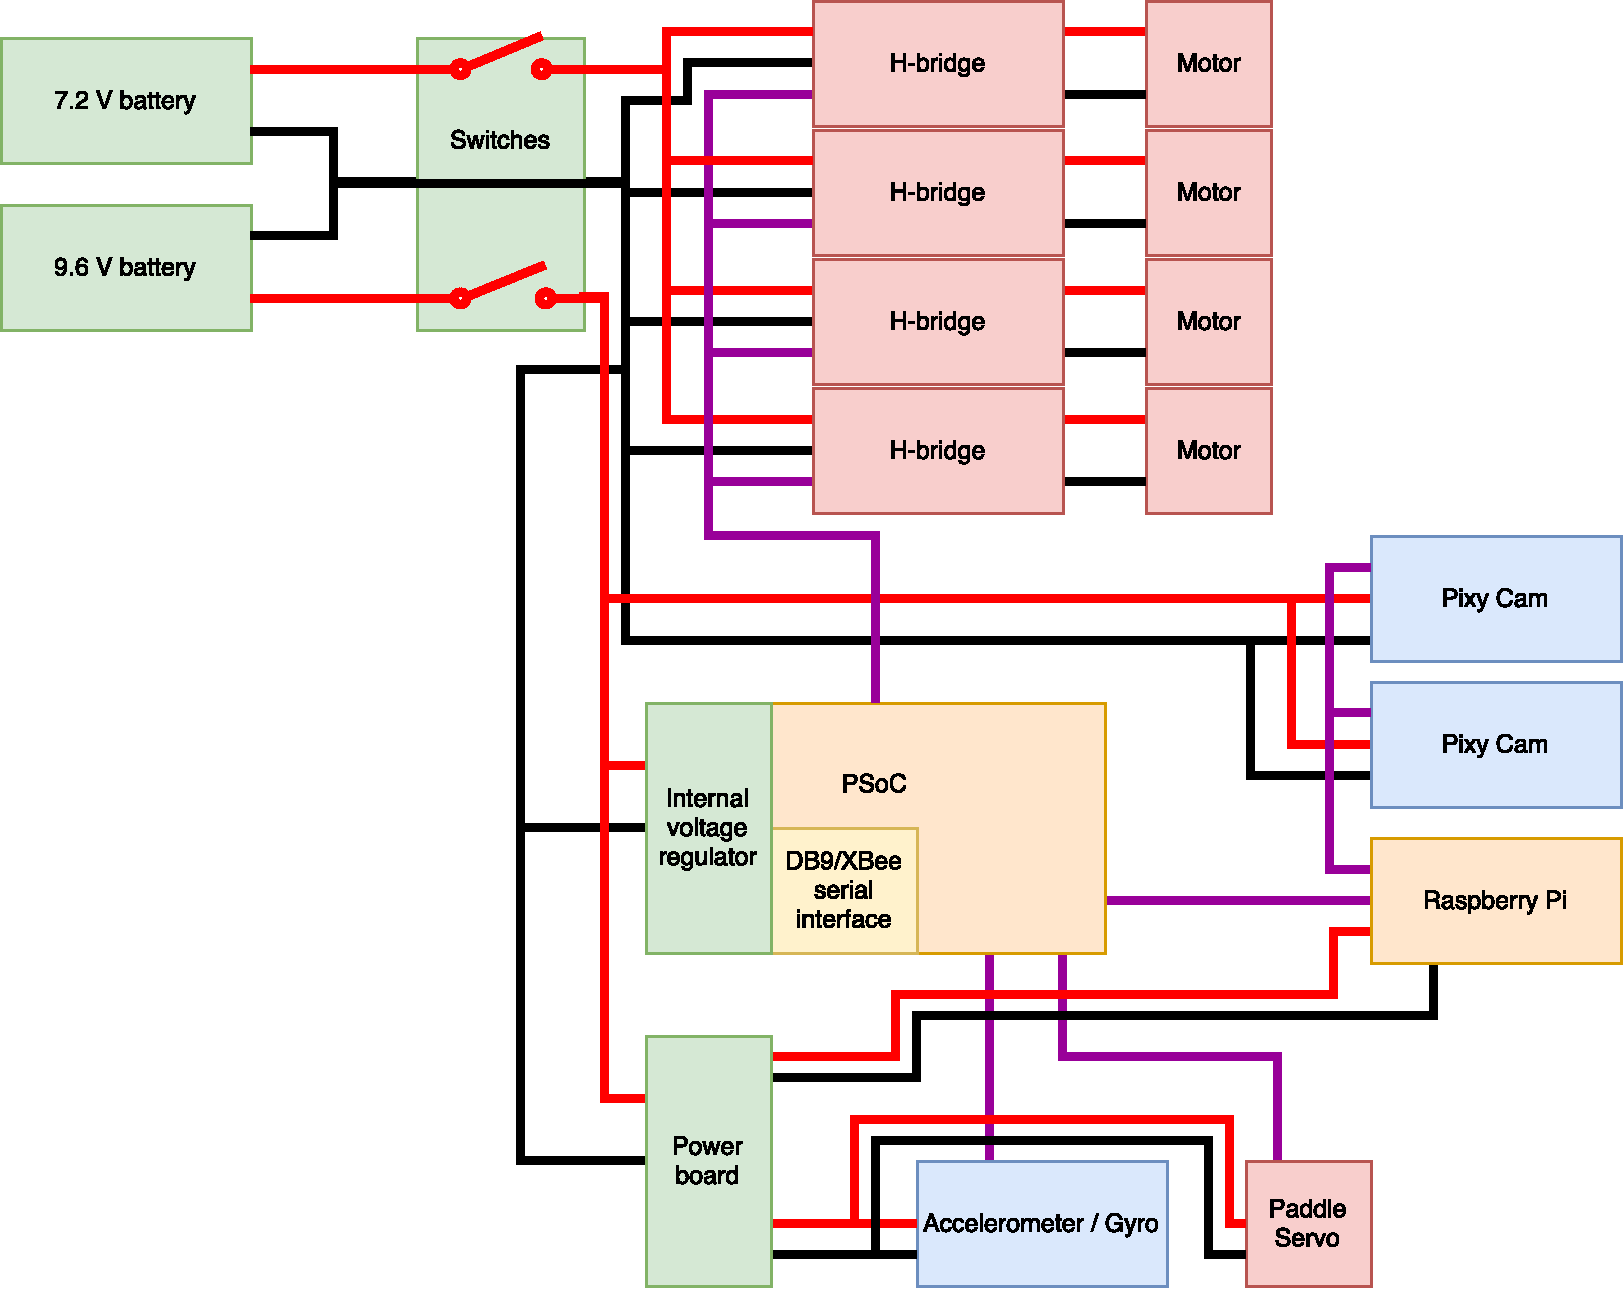
\includegraphics[width=0.85\textwidth]{images/BlockDiagram.pdf}
    \caption{\textbf{Block diagram of the hardware setup for navigation.} Black connections indicate ground connections; red connections indicate power (both regulated and unregulated); all other connections indicate data wires (e.g. from the Hall effect sensor board, to the steering servo and the motor board, and from the camera board). Green components indicate power-related components; red components indicate actuators; blue components indicate sensors.}
    \label{fig:blockdiagram}
\end{figure}

\subsection{Chassis}
%TODO: BC: two decks: lower deck for motors, H bridges, voltage regulator and batteries (we used our own VR because of power requirements); upper deck for RPi, PSoC, accel/gyros
%TODO: BC: figure of laser cut top deck

\subsection{Omni-wheel drive}
%TODO: TJ: what an omni-drive can achieve (i.e. why we needed it), what it requires (independent bidirectional throttled control of four)
\subsubsection{Motors and chassis}
%TODO: TJ: description of motors, chassis (dimensions, components (3D printed components), set screws, etc. - refer to Gordon and Pfleger, 2016), electrical current requirements
\subsubsection{H-bridges and motor control}
%TODO: TJ: description of H-bridges
%TODO: TJ: differences from Gordon and Pfleger (no open-drain comparators)
%TODO: TJ: description of PWM system we used (phase anti-lock? whatever we used)
%TODO: TJ: powered from one 7.2 V NiCd

\subsection{Cameras and mast}
%TODO: BC: camera specifications and details (resoltuion, frame rate, its algorithm and communication protocols)
%TODO: BC: figure of laser cut mast
%TODO: BC: communication protocol

\begin{figure}[ht]
    \centering
    \includegraphics[height=0.3\paperheight,
                     angle=0, origin=c]{images/MastLabeled.jpg}
    \caption{\textbf{Camera mounted on mast.} Labels indicate the mast, the camera and the cable connecting the camera to the camera board.}
    \label{fig:mast}
\end{figure}


\subsection{Paddle mount}
%TODO: TJ: CAD models and servo specifications

\begin{figure}[ht]
    \centering
    \begin{subfigure}[b]{0.45\textwidth}
        \centering
        \includegraphics[height=3in,
                         angle=0, origin=c]{images/CameraBoard.JPG}
        \caption{Photograph}
    \end{subfigure}%
    \begin{subfigure}[b]{0.55\textwidth}
        \centering
        \includegraphics[height=3in,
                         trim=0 0 0 0, clip]{images/CameraBoard.pdf}
        \caption{Schematic}
    \end{subfigure} \\ \vspace{1cm}
    \begin{subfigure}[b]{0.99\textwidth}
        \centering
        \includegraphics[width=\textwidth,
                         trim=0 0 0 0, clip]{images/CameraBoard_circuit.pdf}
        \caption{Circuit diagram}
    \end{subfigure}
    \caption{\textbf{Circuitry of the camera board.}}
    \label{fig:cameraboard}
\end{figure}

\subsection{Power supply}
%TODO: BC: voltage regulators
%TODO: BC: supplying power to the rpi, and difficulties we had

\subsection{Programmable hardware}
%TODO: BC: topdesign
Figure~\ref{fig:topdesign} shows the top-design of our programmable hardware in PSoC Creator 2.1.
\begin{figure}[ht]
    \centering
    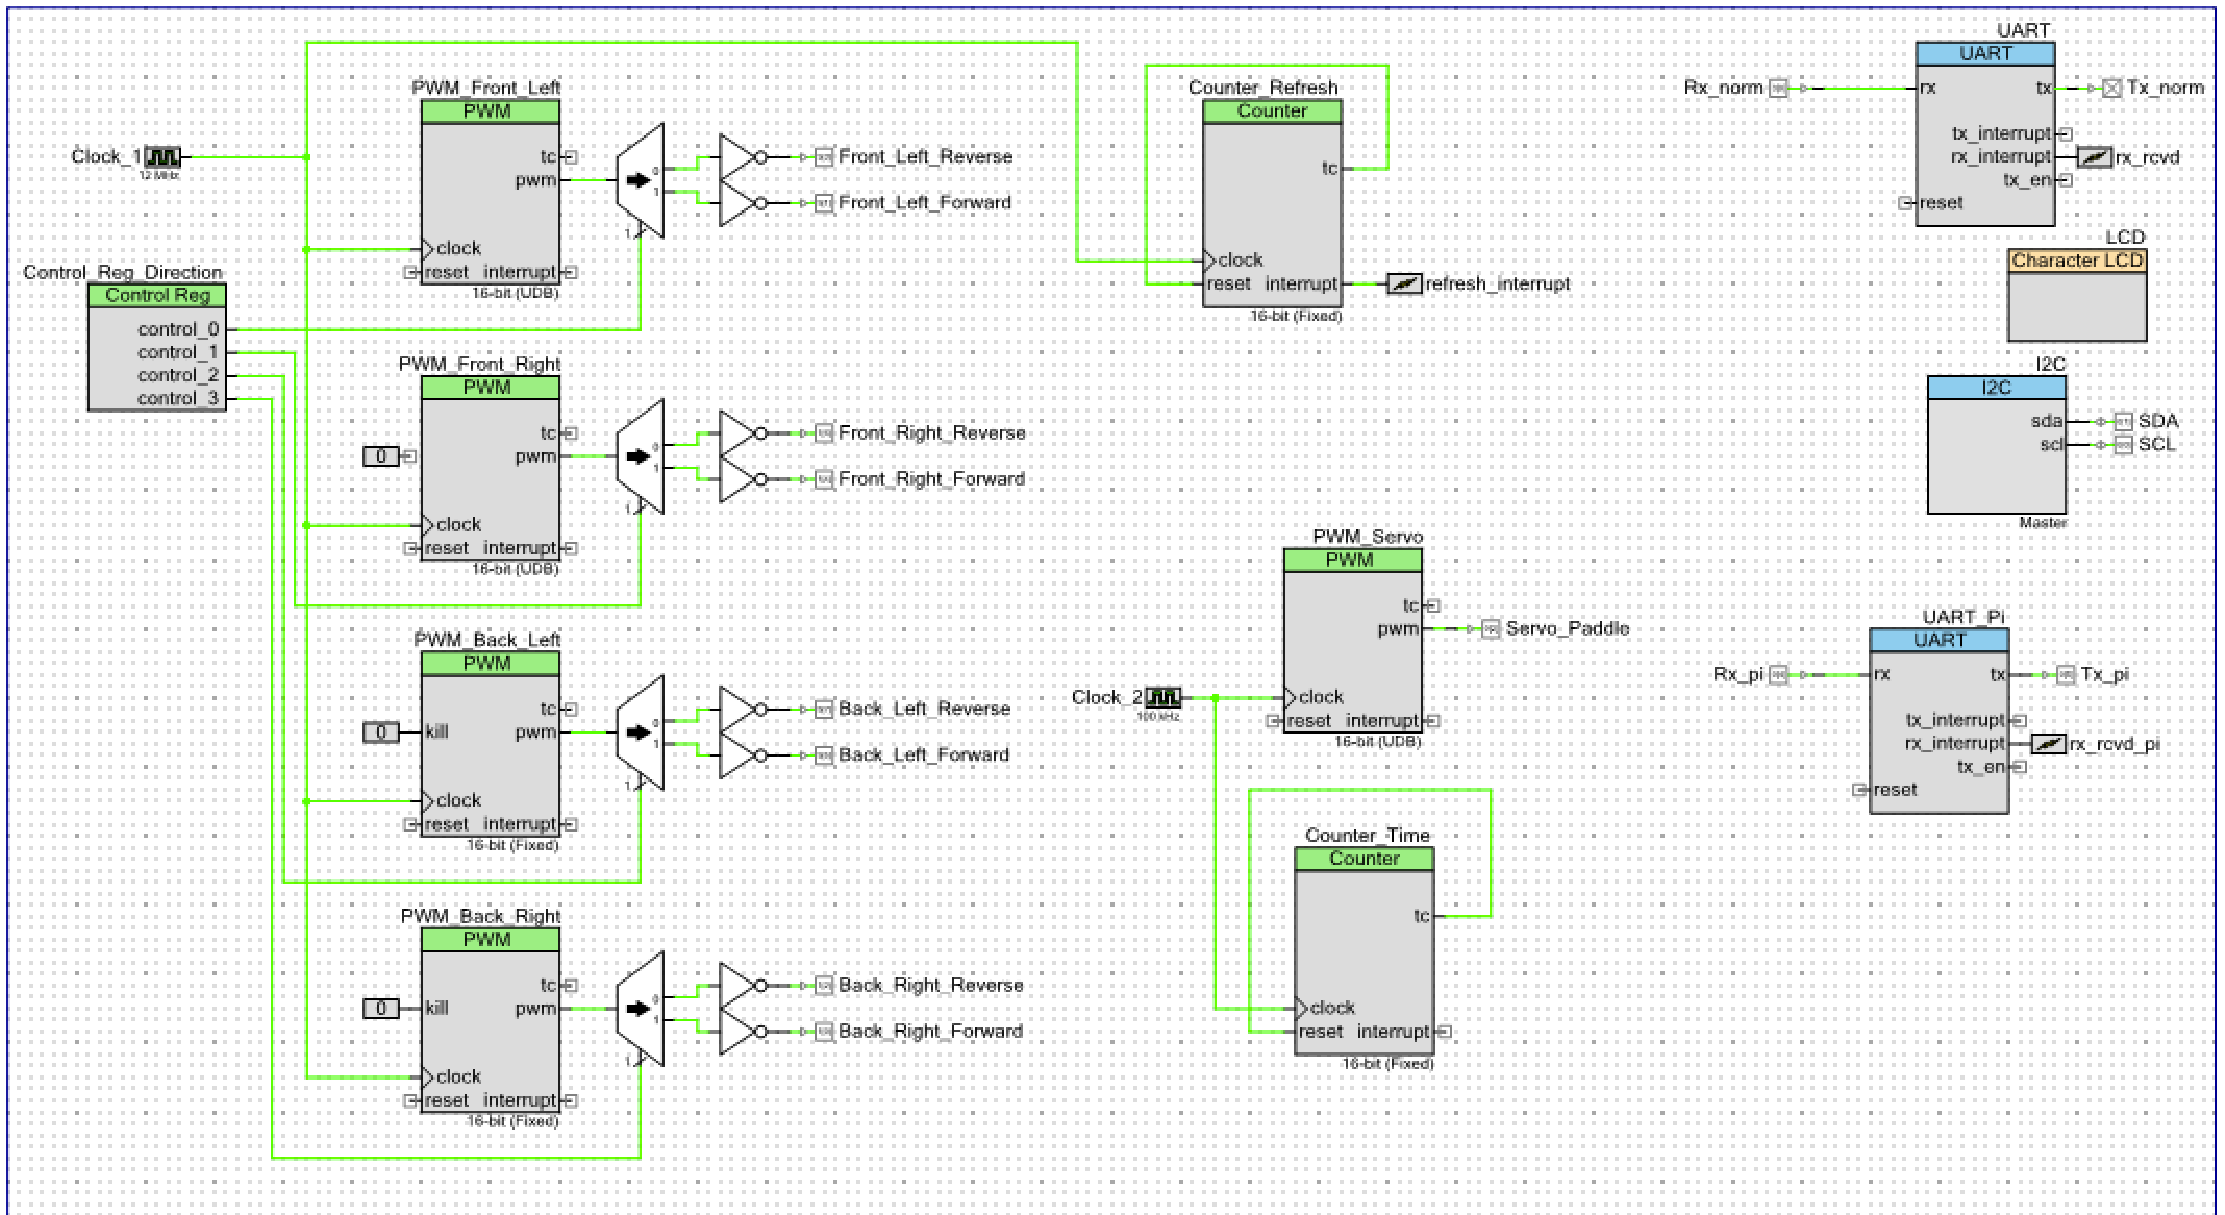
\includegraphics[height=0.99\textwidth,
                     angle=-90, origin=c,
                     trim=1.2in 1in 1.8in 1in, clip]{images/topdesign.pdf}
    \vspace*{-3cm}
    \caption{\textbf{Top-design of the navigation project.}}
    \label{fig:topdesign}
\end{figure}

\subsubsection{Hardware for motor control}
%TODO: TJ

\subsubsection{Hardware for dead reckoning}
%TODO: TJ

\section{Software for PSoC}

\subsection{Omni-drive control}
%TODO: TJ

\subsection{Dead reckoning}
%TODO: TJ

\subsection{Paddle mount servo control}
%TODO: TJ

\section{Software for Raspberry Pi}
\subsection{Pixy camera communication}
%TODO: BC

\subsection{Stereo vision}
%TODO: BC

\subsection{Trajectory estimation}
%TODO: BC

\subsection{Serial communication}
%TODO: update (TJ)
We continued to use serial communication extensively to debug the camera and navigation portions of our program and to adjust our PID variables. We also moved to using the DB9 header only for bench testing and a wireless XBee serial communication chip for track testing. We changed nearly no code or programmable hardware to move to the XBee, since it relied on the same UART communication as the DB9.

We heavily updated our list of serial commands to improve memorability and consistency, and to expand to control camera and navigation parameters. Our updated commands are listed in Table~\ref{tbl:commands}.
\begin{table}[ht]
    \centering
    \begin{tabular}{@{}ll@{}}
        \toprule
        \textbf{Command} & \textbf{Description} \\ \midrule
        \texttt{CTx} & Change throttle \\
        \texttt{GS} & Get all variables associated with speed control \\
        \texttt{TS} & Toggle speed PID control \\
        \texttt{TDC} & Toggle distance timeout for speed control \\
        \texttt{TDS} & Toggle dynamic speed control \\
        \texttt{CPSx} & Change proportional term for speed control \\
        \texttt{CISx} & Change integral term for speed control \\
        \texttt{CDSx} & Change derivative term for speed control \\
        \texttt{CSSx} & Change steady-state throttle for speed control \\
        \texttt{CTSx} & Change target speed for speed control \\
        \texttt{CTDx} & Change target distance for speed control \\
        \texttt{TVS} & Toggle verbose printout for speed PID control \\ \midrule
        \texttt{GC} & Get all camera variables \\
        \texttt{RC} & Reset camera variables \\
        \texttt{CSx} & Change steering/servo direction \\
        \texttt{CMMx} & Change maximum permitted line misses \\ \midrule
        \texttt{TN} & Toggle navigation PID control \\
        \texttt{CPLx} & Change proportional term for line position error \\
        \texttt{CILx} & Change integral term for line position error \\
        \texttt{CIILx} & Change double integral term for line position error \\
        \texttt{CDLx} & Change derivative term for line position error \\
        \texttt{CPTx} & Change proportional term for angle error \\
        \texttt{CITx} & Change integral term for angle error \\
        \texttt{CDTx} & Change derivative term for angle error \\
        \texttt{CTSNx} & Change nominal target speed for navigation \\
        \texttt{TLE} & Toggle line error tracking \\
        \texttt{TVN} & Toggle verbose printout for navigation PID control \\ \midrule
        \texttt{A} & Abort (kill speed and navigation PID control) \\ \bottomrule
    \end{tabular}
    \caption{\textbf{Table of serial interface commands.}}
    \label{tbl:commands}
\end{table}

\section{Results}
See Table~\ref{tbl:pid} for the final PID coefficients we used. We updated our coefficients from speed control because we are no longer dynamically updating the target speed to reach the distance in a specific time. We used only the proportional and derivative terms for line position and angle (no integral terms), and unfortunately, despite our efforts to calculate it accurately, the angle contributed very little to our control. Given more time, we may have been able to develop a better system of control to more robustly control steering at higher speeds.
\begin{table}[ht]
    \centering
    \begin{tabular}{@{}rlll@{}}
        \toprule
        & \textbf{P} & \textbf{I} & \textbf{D} \\ \midrule
        Speed control & $80.0$ & $1.0$ & $10.0$ \\
        Line position & $3.0$ & $0.0$ & $2.0$ \\
        Line angle & $0.5$ & $0.0$ & $0.0$ \\ \bottomrule
    \end{tabular}
    \caption{\textbf{Final PID coefficients}}
    \label{tbl:pid}
\end{table}

See Table~\ref{tbl:times} for our final times for one lap. The highest speed we managed to achieve was with a nominal \SI{6.0}{ft/s}, though by reducing speed while turning corners, our average speed was only about \SI{5.4}{ft/s}. We were unfortunately unable to consistently replicate this speed, and we performed our demo with a nominal target speed of \SI{4.0}{ft/s}.
\begin{table}[ht]
    \centering
    \begin{tabular}{@{}lll@{}}
        \toprule
        \textbf{Nominal target speed} & \textbf{Time for one lap} & \textbf{Average lap speed} \\ \midrule
        \SI{4.0}{ft/s} & \SI{28}{s} & \SI{3.8}{ft/s} \\
        \SI{5.0}{ft/s} & \SI{22}{s} & \SI{4.9}{ft/s} \\
        \SI{6.0}{ft/s} & \SI{19.96}{s} & \SI{5.4}{ft/s} \\ \bottomrule
    \end{tabular}
    \caption{\textbf{Time trial results}}
    \label{tbl:times}
\end{table}

\section{Further work}
%TODO: BC: more robust ball tracking, more robust movement accuracy and location tracking, more robust UART communication, some sort of PID control with global coordinates and camera coordinates so that position could be updated in real time

\clearpage
\section{Appendix: full listings}
\etocsetnexttocdepth{2}
\etocsettocstyle{\subsection*{Contents}}{}
\cftsubsubsecindent 0pt
\localtableofcontents

\subsection{\texttt{main.c}}
% \begin{mdframed}[backgroundcolor=bg]
%     \inputminted[breaklines]{c}{files/main.c}
% \end{mdframed}


\end{document}
